\documentclass[10pt,a4paper]{article}
\usepackage[margin=2.2cm]{geometry}
\usepackage{fontspec}
\usepackage{kotex}
\setmainfont{Apple SD Gothic Neo}
\setsansfont{Apple SD Gothic Neo}
\usepackage{amsmath,amssymb}
\usepackage{graphicx}
\usepackage{booktabs}
\usepackage{caption}
\usepackage[dvipsnames]{xcolor}
\usepackage[colorlinks=true,linkcolor=MidnightBlue,citecolor=MidnightBlue,
            urlcolor=MidnightBlue]{hyperref}
\usepackage{titlesec}
\titleformat{\section}{\large\bfseries}{\thesection}{0.6em}{}
\titleformat{\subsection}{\normalsize\bfseries}{\thesubsection}{0.5em}{}
\captionsetup{font=small,labelfont=bf}
\setlength{\parskip}{0.35em}
\setlength{\parindent}{0pt}

\usepackage{mdframed}
\newmdenv[linewidth=0.4pt,linecolor=gray!60,backgroundcolor=gray!5,
          innertopmargin=6pt,innerbottommargin=6pt,skipabove=8pt,skipbelow=8pt]{claimbox}
\newcommand{\claim}[2]{\begin{claimbox}\textbf{주장.} #1\par\smallskip
  \textcolor{gray!70}{\textbf{반증 조건.} #2}\end{claimbox}}

\title{\bfseries 계열은 없었다\\[2pt]
\large 한 시간 전에 낸 논문의 결론을 행수 맞춘 팔이 반증했다}
\author{월드모델 실험실 · 노트 724 · 725 (논문 142 정정)}
\date{2026-08-06}
\begin{document}\maketitle

\section{한 줄}

\textbf{논문 142 가 \emph{``공유 표현은 하나의 IP 계열 안에서만 옮겨간다''}로 나갔다.}
그 논문 자체가 \emph{``계열과 크기가 교란돼 있어 이 자료로는 못 가른다''}를 반증
조건으로 적었고, 그 실험을 바로 돌렸다. \textbf{계열이 죽었다} --- 계열 안 학습이
문턱 밖으로 이기는 것은 $4/11$ 이고 \textbf{그 넷이 계열로 묶이지 않는다.}
그리고 \textbf{크기도 답이 아니다.}

\section{무엇을 가려야 했나}

노트 723 은 LODO(전부 $-$ 자기)로 \textbf{일본 만화·애니 셋만 양수}를 쟀다
(애니 $+0.1411$ · 세계애니 $+0.0581$ · 만화 $+0.0164$ · 나머지 여덟 음수). 그런데
\textbf{LODO $\leftrightarrow$ 학습 행수 스피어만이 $+0.818$}($p{=}0.002$)이고
\textbf{큰 도메인이 곧 그 계열}이다. ``계열이라 옮겨간다''와 ``풀이 커서
옮겨간다''가 구분되지 않았다.

\subsection*{설계 --- 셋째 팔이 식별을 준다}

목표 도메인 $d$ 마다 트렁크를 셋 적합했다.

\begin{center}
\begin{tabular}{ll}
\toprule
\textbf{계열 안} & $d$ 의 형제만으로 학습($d$ 자신 제외) \\
\textbf{계열 밖} & 계열이 다른 도메인만으로 \\
\textbf{계열 밖 · 행수 맞춤} & 계열 밖에서 \textbf{계열 안과 같은 행수}만 뽑아 \\
\bottomrule
\end{tabular}
\end{center}

\textbf{셋째가 없으면 아무것도 못 가른다} --- 웹툰의 계열 안은 $196$행이고 계열 밖은
$15{,}325$행이라 크기만으로 계열 밖이 이긴다.

\begin{figure}[t]\centering
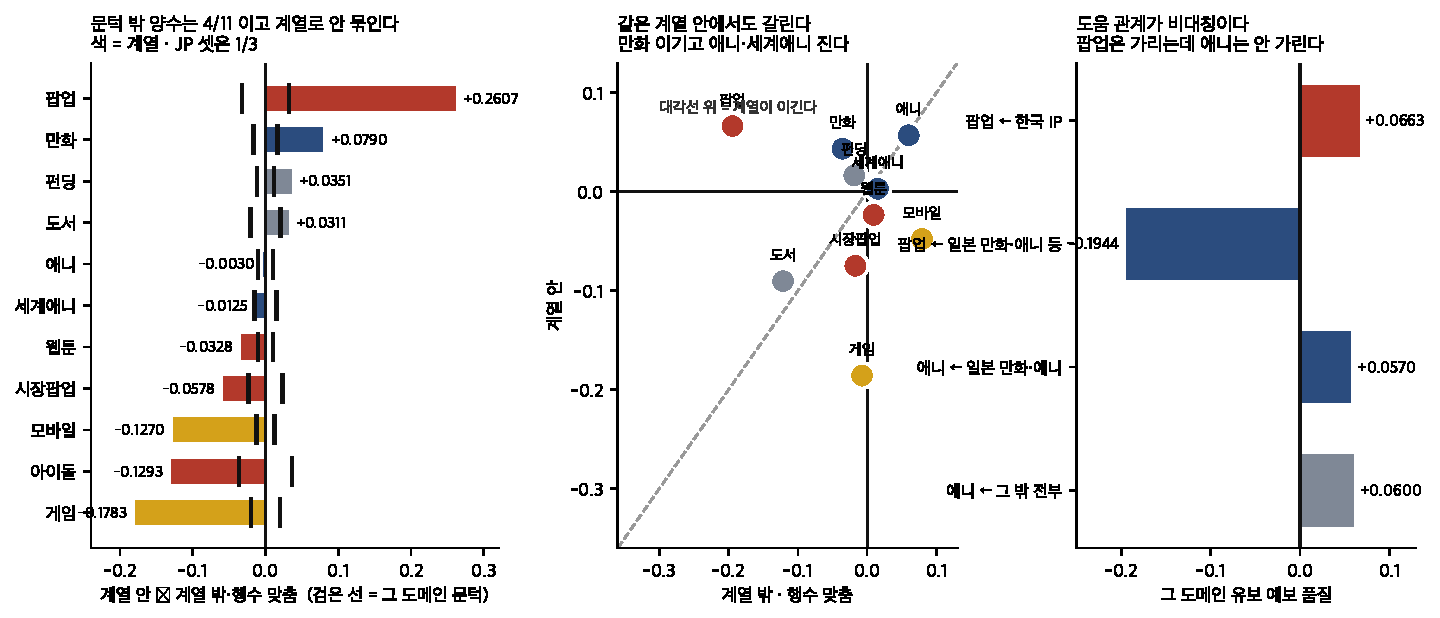
\includegraphics[width=0.99\textwidth]{figs/nofamily.pdf}
\caption{왼쪽: 계열 안 $-$ 밖·맞춤. \textbf{문턱(검은 선) 밖 양수는 $4/11$ 이고
색(계열)이 섞여 있다.} 가운데: 같은 계열 안에서도 갈린다. 오른쪽: \textbf{도움
관계가 비대칭이다.}}
\end{figure}

\section{계열이 죽었다}

\begin{center}
\begin{tabular}{lrrrrl}
\toprule
도메인 & 계열 안 & 밖·맞춤 & \textbf{안 $-$ 맞춤} & 문턱 & 계열 \\
\midrule
팝업 & $+0.0663$ & $-0.1944$ & $\mathbf{+0.2607}$ & $0.0324$ & 한국 IP \\
만화 & $+0.0435$ & $-0.0355$ & $\mathbf{+0.0790}$ & $0.0163$ & 일본 만화·애니 \\
펀딩 & $+0.0165$ & $-0.0186$ & $\mathbf{+0.0351}$ & $0.0114$ & 그밖 \\
도서 & $-0.0903$ & $-0.1214$ & $\mathbf{+0.0311}$ & $0.0205$ & 그밖 \\
\midrule
애니 & $+0.0570$ & $+0.0600$ & $-0.0030$ & $0.0106$ & 일본 만화·애니 \\
세계애니 & $+0.0030$ & $+0.0155$ & $-0.0125$ & $0.0151$ & 일본 만화·애니 \\
웹툰 & $-0.0234$ & $+0.0094$ & $-0.0328$ & $0.0102$ & 한국 IP \\
시장팝업 & $-0.0748$ & $-0.0170$ & $-0.0578$ & $0.0233$ & 한국 IP \\
모바일 & $-0.0478$ & $+0.0792$ & $-0.1270$ & $0.0124$ & 앱·게임 \\
아이돌 & $-0.4529$ & $-0.3236$ & $-0.1293$ & $0.0366$ & 한국 IP \\
게임 & $-0.1857$ & $-0.0074$ & $-0.1783$ & $0.0195$ & 앱·게임 \\
\bottomrule
\end{tabular}
\end{center}

사전등록 예측은 \emph{``JP 셋에서 $3/3$ 양수''}였다. 실측은 \textbf{$1/3$} --- 만화만
이기고 애니 $-0.0030$ · 세계애니 $-0.0125$ 다.

\claim{\textbf{계열 안이 문턱 밖으로 이기는 넷이 계열로 묶이지 않는다} --- 한국 IP
하나(팝업) · 일본 만화·애니 하나(만화) · 그밖 둘(펀딩 · 도서). \textbf{같은 계열
안에서도 갈린다}(만화 $+0.0790$ 대 애니 $-0.0030$ · 팝업 $+0.2607$ 대 아이돌
$-0.1293$). 그러므로 논문 142 의 \emph{``하나의 IP 계열 안에서만 옮겨간다''}는
\textbf{철회한다.}}
{계열 묶기가 내 눈이 정한 것이므로 \emph{다른} 묶기에서는 설 수 있다. 그러나
그것은 자료가 정하게 해야 하고(군집), 그때는 ``내가 아는 계열''이 아니라 ``자료가
찾은 무리''라는 다른 주장이 된다.}

\subsection*{크기도 답이 아니다}

행수를 맞춘 팔이 \textbf{이기기도 지기도} 한다 --- 모바일에서 $+0.0792$ 로 계열 안을
크게 이기고 팝업에서 $-0.1944$ 로 크게 진다. \textbf{형제 학습행으로도 유보
행수로도 무늬가 없다.}

\subsection*{배선 한계 --- 정직하게}

\textbf{애니와 세계애니에서는 ``행수 맞춤''이 맞출 게 없었다.} 형제 학습행이
$8{,}291$ · $8{,}423$ 인데 계열 밖이 $7{,}387$ · $7{,}255$ 라 뽑을 것이 전부였고,
그래서 그 두 줄은 \textbf{``계열 밖''과 ``밖·맞춤''이 정확히 같다}. 행수가 $1.12$ ·
$1.16$배로 가까우므로 비교는 유효하지만 \textbf{엄밀한 통제는 아니다}. 만화는 형제
$5{,}426$ 대 계열밖 $10{,}252$ 라 맞춤이 실제로 작동했다.

\section{남는 것 --- 계열이 아니라 짝이고, 비대칭이다}

가장 큰 값이 \textbf{팝업 $+0.2607$}(문턱의 $8$배)이다. 팝업의 계열 안(웹툰 $+$
시장팝업 $+$ 아이돌 $3{,}115$행)이 $+0.0663$ 을 주고 계열 밖은 $\mathbf{-0.1944}$ 를
준다 --- \textbf{팝업에게 다른 계열은 크게 해롭다.} 그런데 \textbf{역이 성립하지
않는다} --- 애니는 계열 안 $+0.0570$ 과 계열 밖 $+0.0600$ 이 같다.

\claim{\textbf{도움 관계가 비대칭이다.} 어떤 도메인은 무엇을 같이 학습하느냐에 크게
흔들리고(팝업 $0.26$ 폭) 어떤 도메인은 거의 안 흔들린다(애니 $0.003$ 폭).
\textbf{그러므로 설계 물음이 ``무엇을 같이 학습하나''에서 ``무엇을 소스로
쓰나''로 바뀐다.}}
{$11\times11$ 짝별 전이 행렬이 대칭으로 나오면 이 주장이 틀리고, 그때는 ``비슷한
도메인끼리''라는 그림이 선다. 그 측정을 이 논문과 동시에 걸었다.}

\subsection*{그리고 노트 723 의 교란 정체가 바뀐다}

노트 723 의 셋이 양수였던 이유를 나는 ``계열''로 읽었다. 노트 725 가 그것을
반증했으므로 남는 설명은 \textbf{그 도메인들의 라벨이 텍스트로 예측 가능해서}다
--- LODO $\leftrightarrow$ 학습 행수 $+0.818$ 이 같은 방향을 가리킨다.
\textbf{즉 교란의 정체가 ``계열''이 아니라 ``예측 가능성''이다.}

\claim{\textbf{한 시간 만에 자기 논문을 깎았다 --- 그것이 반증 조건을 적어 두는
값이다.} 논문 142 는 결론과 함께 \emph{``계열과 크기가 교란돼 있어 못 가른다''}를
적었고, \textbf{그 문장이 다음 실험을 지정했다.} 반증 조건이 없었다면 계열 이야기가
남았을 것이다.}
{반증 조건을 적어도 그 실험을 안 돌리면 아무 소용이 없다. 이 실험이 싼 이유는
트렁크가 $2{,}497$ 모수라 적합이 4초이기 때문이다 --- \textbf{비싼 실험에서는 같은
규율이 안 지켜질 수 있고, 그것이 이 판의 진짜 위험이다.}}

\end{document}
